\documentclass{article}
\usepackage[margin=1in]{geometry}
\usepackage{tikz}
\usetikzlibrary{positioning}

\begin{document}

\begin{center}
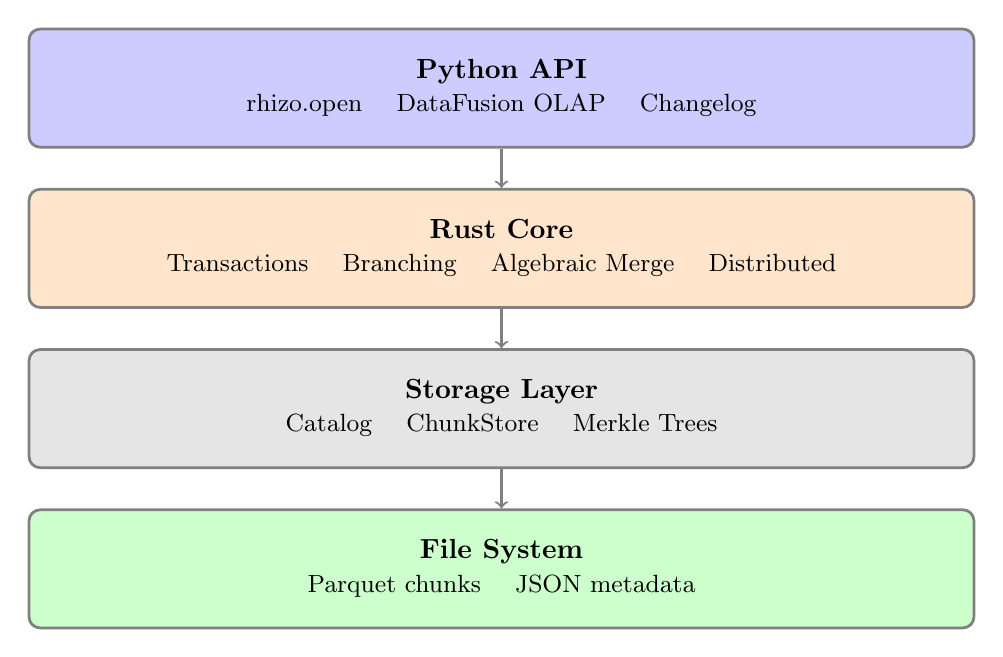
\begin{tikzpicture}

% Python API Layer
\node[rectangle, rounded corners, minimum width=12cm, minimum height=1.5cm,
      draw=gray, fill=blue!20, line width=1pt] (python) at (0,0) {
  \begin{tabular}{c}
    \textbf{Python API} \\
    \small rhizo.open \quad DataFusion OLAP \quad Changelog
  \end{tabular}
};

% Rust Core Layer
\node[rectangle, rounded corners, minimum width=12cm, minimum height=1.5cm,
      draw=gray, fill=orange!20, line width=1pt, below=0.5cm of python] (rust) {
  \begin{tabular}{c}
    \textbf{Rust Core} \\
    \small Transactions \quad Branching \quad Algebraic Merge \quad Distributed
  \end{tabular}
};

% Storage Layer
\node[rectangle, rounded corners, minimum width=12cm, minimum height=1.5cm,
      draw=gray, fill=gray!20, line width=1pt, below=0.5cm of rust] (storage) {
  \begin{tabular}{c}
    \textbf{Storage Layer} \\
    \small Catalog \quad ChunkStore \quad Merkle Trees
  \end{tabular}
};

% File System Layer
\node[rectangle, rounded corners, minimum width=12cm, minimum height=1.5cm,
      draw=gray, fill=green!20, line width=1pt, below=0.5cm of storage] (fs) {
  \begin{tabular}{c}
    \textbf{File System} \\
    \small Parquet chunks \quad JSON metadata
  \end{tabular}
};

% Arrows
\draw[->, thick, gray] (python.south) -- (rust.north);
\draw[->, thick, gray] (rust.south) -- (storage.north);
\draw[->, thick, gray] (storage.south) -- (fs.north);

\end{tikzpicture}
\end{center}

\end{document}
